\chapter{\IfLanguageName{dutch}{Stand van zaken}{State of the art}}
\label{ch:stand-van-zaken}

% Tip: Begin elk hoofdstuk met een paragraaf inleiding die beschrijft hoe
% dit hoofdstuk past binnen het geheel van de bachelorproef. Geef in het
% bijzonder aan wat de link is met het vorige en volgende hoofdstuk.

% Pas na deze inleidende paragraaf komt de eerste sectiehoofding.
\section{\IfLanguageName{dutch}{Inleiding}{Preface}}
\label{sec:standvanzaken-inleiding}

Deze bachelorproef onderzoekt of machine learning engines gebruikt kunnen worden voor het automatisch classificeren van afbeeldingen. In deze stand van zaken komen volgende onderwerpen aan bod:
\begin{enumerate}
    \item Classificeren van afbeeldingen: terminologie en technieken
    \item Bespreking belangrijkste stromingen binnen machine learning
    \item Computer vision: hoe wordt classificatie en machine learning gecombineerd
\end{enumerate}

\section{\IfLanguageName{dutch}{Classificeren van afbeeldingen}{Image classification}}
\label{sec:classificeren-van-afbeeldingen}
Voor er dieper in gegaan wordt op machine learning en hoe deze algoritme's kunnen toegepast worden om computers te laten 'zien' is het belangrijk om te bespreken hoe classificatie van afbeeldingen gebeurt.

Het classificeren van afbeeldingen kan gedefinieerd worden als het groeperen van afbeeldingen in semantisch betekenisvolle categorien op basis van onderdelen van de afbeeldingen \autocite{Vailaya1998}. Deze ''semantisch betekenisvolle categorieën'' worden ook labels genoemd, voorbeelden van labels zijn 'fiets', 'landschap', 'blijdschap'. Het is belangrijk om te vermelden dat labels zowel objecten kunnen zijn maar ook meer algemene of abstracte concepten. Verder kunnen labels meer of minder gedetailleerd zijn, denk bijvorbeeld aan 'mens'; 'gezicht'; 'oog'; 'pupil'; ... Het correct aanduiden van labels is een belangrijk probleem wanneer men grote datasets van afbeeldingen zoekbaar wilt maken, bijvoorbeeld foto-archieven of medisch beeldmateriaal. Deze labels worden typisch niet in de afbeelding zelf opgeslaan maar in een bijhorend metadata bestand; wanneer er metadata voor een afbeelding beschikbaar is spreekt men van een verrijkte afbeelding.

Naast het zoeken van labels voor een afbeelding kan men ook eventuele tekst op de afbeelding lezen en deze toevoegen aan de metadata, opnieuw wordt op deze manier de afbeelding verrijkt. Bijvoorbeeld het woord 'Politie' bij een foto van een politie-kantoor.

In de volgende secties wordt manuele (of mens-gestuurde) en automatische (of computer-gestuurde) classificatie meer in detail besproken.

\subsection{\IfLanguageName{dutch}{Manuele classificatie}{Manual classification}}
\label{sec:manuele-classificatie}
Manuele classificatie wordt gedefinieerd als het toewijzen van labels aan een afbeelding, uitgevoerd door een mens. Het manueel classificeren van afbeeldingen is een tijdrovend proces. Iedere afbeelding moet door een persoon geopend worden, deze persoon bekijkt de afbeelding en verrijkt de afbeelding aan de hand van labels. Voor het classificeren van miljoenen of miljarden afbeeldingen is manuele classificatie zeer tijdsintensief en wordt er vaak naar automatische opties gezocht. Automatische of computergestuurde modellen hebben echter steeds manueel gelabelde datasets als trainingsmateriaal dus is het cruciaal dat de kwaliteit van deze manueel geclassificeerde datasets hoog is \autocite{JuliaMoehrmann2012}.

Er werd reeds veel onderzoek en ontwikkeling verricht naar hoe men mensen kan helpen afbeeldingen op een snelle en correcte manier te labelen. Bijvoorbeeld via geavanceerde interfaces \autocite{JuliaMoehrmann2012} of gamification \autocite{LuisvonAhn2004}. Een voorbeeld van manuele classificatie is het invullen van een CAPTCHA, de manuele input van deze beveiligingstechnologie wordt door Google gebruikt om machine learning modellen te trainen \autocite{Google2021}, zie Figuur~\ref{fig:captcha}.

\begin{figure}
    \centering    
    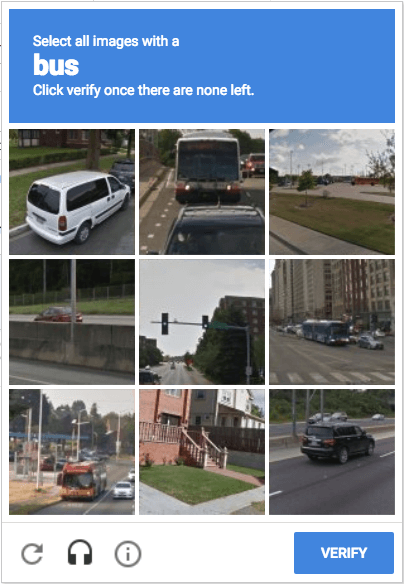
\includegraphics[scale=0.5]{recaptcha}
    \caption{CAPTCHA's worden als input gebruikt voor machine learning modellen. Bron: \url{https://auth0.com/blog/captcha-can-ruin-your-ux-here-s-how-to-use-it-right}}
    \label{fig:captcha}
\end{figure}

\subsection{\IfLanguageName{dutch}{Automatiche classificatie}{Automatic classification}}
\label{sec:automatic-classification}
Onder automatische classificatie begrijpen we het toewijzen van labels aan een afbeelding zonder menselijke input. Een computermodel krijgt een afbeelding aangeboden en wijst aan deze afbeelding verschillende labels toe. Aan iedere label zal een zekerheidsgraad meegegeven worden, uitgedrukt in procent. De computermodellen worden steeds getraind op basis van manueel geclassificeerde afbeeldingen, ook controle van de resultaten gebeurt door menselijke supervisie. Er is dus steeds een samenwerking tussen mens en machine. Typisch worden er machine learning modellen gebruikt om automatische classifictie zo correct mogelijk toe te passen.

Bij het automatisch classificeren van afbeeldingen kan men ook Optical Character Recognition (OCR) uitvoeren. OCR engines zullen proberen tekst te herkennen op een afbeelding en deze toevoegen aan de metadata. Het uitvoeren van kwalitatieve OCR is een apart vakgebied binnen machine learning waar er de laatste jaren veel vooruitgang werd geboekt, een belangrijk probleem in dit veld is het herkennen van handgeschreven tekst \autocite{Breuel2013}.

\section{\IfLanguageName{dutch}{Machine learning}{machine learning}}
\label{sec:machine-learning}
Machine learning is een bepaalde soort computer algoritme dat ontworpen werd om menselijke intelligentie te emuleren door bij te leren uit de directe omgeving \autocite{ElNaqa2015}. Op basis van vroegere ervaringen zal het algoritme trachten om efficientie te verhogen of correcte voorspellingen te maken. In deze context wordt ervaring gedefinieerd als informatie die voor het systeem beschikbaar is, typisch in de vorm van elektronische data. Deze elektronische data kan verschillende vormen aannemen, bijvoorbeed datasets gelabeld door mensen of data gegeneerd door andere machines op basis van hun contact met de buitenwereld. De hoeveelheid en kwaliteit van de data zal steeds cruciaal zijn voor de performantie van het machine learning algoritme \autocite{Mohri2018}.

Machine learning algoritmes bieden computer de mogelijkheid om te leren zonder expliciet geprogrammeerd te zijn \autocite{DeVreese2017}. De problemen waarvoor machine learning meestal gebruikt wordt zijn te complex om via klassieke programmeertechnieken aan te pakken. Aangezien machine learning slechts een techniek is waarmee men tracht complexe problemen op te lossen werd het succesvol gebruikt in uiteenlopende onderzoeksvelden zoals ruimtevaart, statistiek, biomedica en computer vision.

Machine learning algoritmes kunnen in het algmeen opgedeeld worden in 3 type's:
\begin{itemize}
    \item Supervised learning
    \item Unsupervised learning
    \item Reinforcement learning
\end{itemize}

\subsection{\IfLanguageName{dutch}{Supervised learning}{Supervised learning}}
\label{sec:supervised-learning}
De belangrijskte karakteristiek van supervised learning is dat het machine learning algoritme een vooraf gelabelde trainingsdataset ter beschikking heeft. Supervised learning zal op basis van deze trainingsdataset trachten, door middel van inductie, modellen op te bouwen die gebruikt kunnen worden om andere ongelabelde datasets te classificeren. Achteraf kan dan gecontroleerd worden hoeveel percent van de nieuwe labels correct werd gevonden en hoe zeker het model was van deze voorspellingen. Zoals de naam van het model aangeeft is er een vorm van een 'supervisor' nodig die het model toont welke labels met welke ervaringen uit de trainingsdata moeten geassocieerd worden \autocite{Cunningham2008}. 

Een voorbeeld van supervised learning is hoe Netflix nieuwe content aan de users voorstelt. Het algoritme start van een gelabelde dataset met daarin de ervaringen van de gebruiker, op basis van deze ervaringen zal het model voorspellingen over nieuwe content maken.

\subsection{\IfLanguageName{dutch}{Unsupervised learning}{Unsupervised learning}}
\label{sec:unsupervised-learning}
In tegenstelling tot supervised learning wordt er bij unsupervised learning vertrokken van een ongelabelde dataset. Het doel is dat het algoritme deze ongelabelde dataset zal intepreteren en een interne representatie van de 'wereld' - de 'wereld' is alle informatie binnen de dataset - zal opbouwen. Een unsupervised learning model zal proberen een diepe kennis van de wereld op te bouwen aan de hand van complexe patroonherkenning \autocite{Hinton1999}. Op basis van deze diepere kennis zal het algoritme de data in verschillende clusters onderverdelen. Analyse van deze clusters kan dan leiden tot het labellen of classificeren van de ongelabelde dataset.

Unsupervised learning wordt in verschillende bedrijfstakken actief toegepast, Google News gebruikt bijvoorbeeld unsupervised learning om nieuwsartikelen rond hetzelfde nieuwsfeit automatisch te clusteren en op een georganiseerde manier aan de gebruiker aan te bieden.

\subsection{\IfLanguageName{dutch}{Reinforcement learning}{Reinforcement learning}}
\label{sec:reinforcement-learning}
Reinforcement learning is een machine learning algoritme dat steeds zal zoeken naar een zo hoog mogelijke beloning, uitgedrukt in een numerieke waarde. Het algoritme krijgt op voorhand geen uitleg wat goed of fout is maar moet zelf ontdekken welke acties leiden tot de grootst mogelijke beloning \autocite{Sutton2018}. Uit het iteratief uitvoeren van dezelfde opdracht en ontvangen van een beloning zal het algoritme een duidelijk beeld krijgen welke acties de grootste beloning opleveren. Het zal steeds een balans moeten houden tussen exploratief onderzoeken en in de diepte onderzoeken van reeds gevonden oplossingen. 

Reinforcement learning vindt toepassingen in verschillende sectoren zoals autonoom auto-rijden, handelen op de aandelenmarkt en gaming. Reinforcement learning sluit inherent dicht aan bij gaming dat met dezelfde soort trial-and-error beloningssystemen werkt, bijgevolg werd er reeds veel onderzoek verricht naar het gebruik van reinforcement learning om spelletjes te spelen. Een voorbeeld uit 2015 is een wedstrijd van het complexe bordspel Go tussen wereldkampioen Fan Hui en AlphaGo. AlphaGo is een algoritme ontwikkeld door Google, gebaseerd op het reinforcement learning principe. Fan Hui verloor de match met 1-4, het was de eerste keer dat een computer-gestuurd programma een Go wereldkampioen versloeg, Figuur~\ref{fig:alphago}.

\begin{figure}
    \centering
    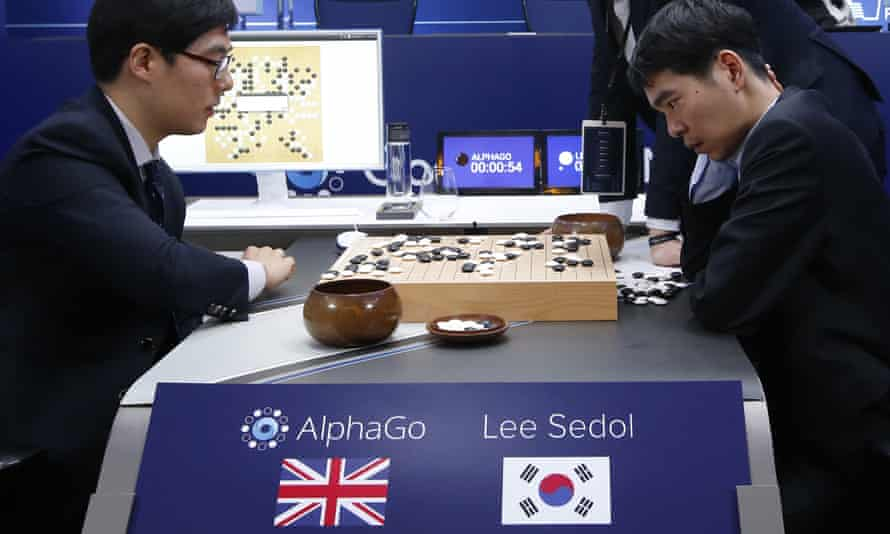
\includegraphics[width=\textwidth]{alphago}
    \caption{Wereldkampioen Fan Hui speelt tegen AlphaGo. Bron: \url{https://www.theguardian.com/technology/2016/mar/15/alphago-what-does-google-advanced-software-go-next}}
    \label{fig:alphago}
\end{figure}

\section{\IfLanguageName{dutch}{Computer vision}{Computer vision}}
\label{sec:computer-vision}
Computer vision wordt begrepen als de combinatie van technieken die gebruikt wordt om complexe hoger-dimensionale data (afbeeldingen) te analyseren en verwerken \autocite{Jaehne2000}. De meest gebruikte machine learning strategieën bij computer vision zijn supervised, unsupervised en semi-supervised \autocite{Khan2020}. Binnen de supervised learning subset wordt computer vision gedefinieerd als een deep learning model. Deep learning betekent dat er gebruikt wordt gemaakt van een neuraal netwerk met ten minste 3 of meer lagen. Een neuraal netwerk is een serie algoritme's die probeert om onderlinge relaties in een dataset te herkennen, het menselijk brein kan ook als een neuraal netwerk gedefinieerd worden.

\subsection{\IfLanguageName{dutch}{Hoe kan een computer 'zien'}{How does a computer 'see'}}
\label{sec:how-do-computer-see}

Voor mensen is zicht en herkenning van de wereld rond ons een normaal en natuurlijk proces. Licht wordt weerkaatst door een object en opgevangen door de ogen, de ogen geven deze data door naar de visuele cortex die het beeld interpreteert. Door middel van miljoenen jaren evolutie werd ons brein getrained in het zien en interpreteren van de wereld. Essentieel is dat iedere mens een bepaald idee heeft van de wereld die de beelden die van de ogen komen betekenis geeft. Dit 'idee van de wereld' wordt ook als context gedefinieerd, zonder context kan een afbeelding geen betekenis hebben.
Bijvoorbeeld als een alien een foto te zien zou krijgen die gemaakt werd op de aarde, zal het voor hem moeilijk zijn om de foto te 'begrijpen' omdat de context ontbreekt.

Het ontbreken van context is wat het voor computers ook heel moeilijk maakt om te herkennen wat er op een afbeelding staat. Voor een computer ziet een afbeelding er typisch uit als Figuur~\ref{fig:pixelarray}, een lijst van integers. De computer weet hoe het deze integers moet omvormen tot een afbeelding, maar heeft geen informatie over de inhoud van de afbeelding.

\begin{figure}
    \centering
    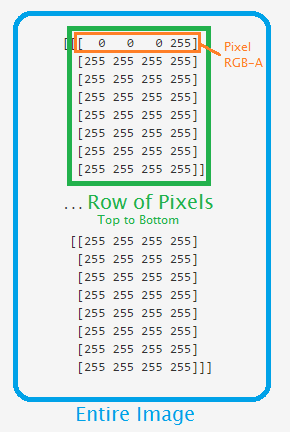
\includegraphics[scale=1]{pixelarray}
    \caption{Voorbeeld van hoe een afbeelding er voor een computer uit ziet. Bron: \url{https://pythonprogramming.net/python-pixel-arrays/}}
    \label{fig:pixelarray}
\end{figure}

Computer vision gebruikt verschillende strategien om context rond een afbeelding op te bouwen, eerst zullen de algoritme's proberen om vormen en figuren te herkennen op de afbeelding. Wanneer deze vormen en figuren gedefinieerd zijn zal men op basis van pre-gelabelde datasets de betekenis van deze figuren afleiden. Op de meeste vlakken heeft computer vision het nadeel van het ontbreken van context, maar in sommige gevallen kan dit net in het voordeel van herkenning spelen. Als men een ingezoomde foto met erop de vacht van een bepaald dier aan een mens toont, zal het vaak moeilijk zijn om het dier te herkennen. Een computer vision algoritme zou kunnen het patroon van de vacht berekenen en op basis hiervan in de pre-geclassificeerde dataset de diersoort opzoeken. Het ontbreken van context speelt hier niet in het nadeel van computer vision.

Na miljoenen jaren natuurlijke evolutie van het zicht zijn we nu op een interessant punt waarbij computer vision steeds dichter bij de menselijke herkenningsskills komt \autocite{Scheirer2014}. In de toekomst zal computer vision waarschijnlijk accurater worden dan het menselijk zicht.

\subsection{\IfLanguageName{dutch}{Convolutional neural network}{Convolutional neural network}}
\label{sec:convolutional-neural-network}
Achterliggend zal men bij computer vision meestal een Convolutional Neural Network (CNN) gebruiken, dit is een bepaald subtype van supervised deep learning. CNN werkt door afbeeldingen op te delen in kleinere groepjes pixels die men filters of feature maps noemt. Deze filters worden door de lagen van het neuraal netwerk doorgegeven, in de eerste lagen zal men proberen om algemene informatie te herkennen zoals randen of vormen. De output van iedere laag wordt aan de volgende doorgegeven, tijdens het doorgeven van het resultaat wordt iedere filter afgecheckt tegen tegen een pre-geclassificeerde trainingsdataset. Het afchecken geeft aan het CNN een bepaalde error-waarde (ofwel loss function) terug, deze error-waarde geeft aan hoe groot de kans is dat er iets herkend wordt. Op basis van deze error-waarde zal het algoritme bij iedere iteratie de filtervalues updaten. Idealiter zal iedere iteratie een betere error-waarde opleveren. Op het einde van het proces wordt alle opgebouwde kennis gepooled tot het herkennen van complexe en abstracte begrippen, zie Figuur~\ref{fig:cnn} voor een overzicht.

\begin{figure}
    \centering
    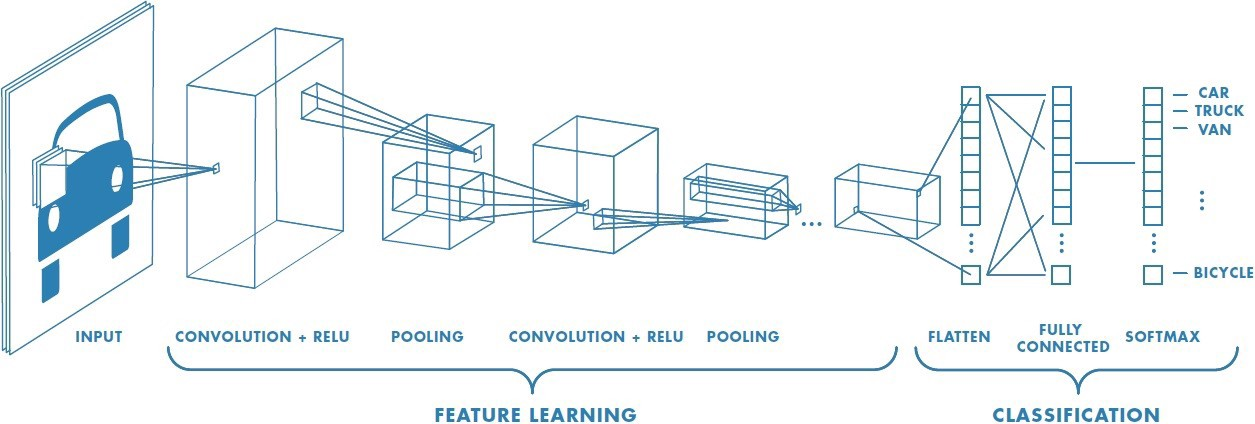
\includegraphics[width=\textwidth]{cnn}
    \caption{Een Convolutional Neural Network (CNN). Bron: \url{https://towardsdatascience.com/a-comprehensive-guide-to-convolutional-neural-networks-the-eli5-way-3bd2b1164a53}}
    \label{fig:cnn}
\end{figure}

Een uitdaging bij dit soort modellen is dat men zeer grote hoeveelheden data nodig heeft (miljoenen afbeeldingen) voor men accuraat labels kan voorspellen \autocite{Chen2014}. Het is belangrijk dat het model van iedere label meerdere voorbeelden heeft, bijvoorbeeld als een model getrained wordt met een afbeelding van een eend en het krijgt slechts 1 afbeelding van een eend; dan zal het model ook de achtergrondkleur en belichting als essentiele informatie van de foto beschouwen. Wanneer men een afbeelding van een andere eend met andere belichting aanbiedt, zal het model dit niet als eend herkennen. Aansluitend is het belangrijk dat de trainingsdataset correct gelabeld is.

\subsection{\IfLanguageName{dutch}{Recurrent neural network}{Recurrent neural network}}
\label{sec:recurrent-neural-network}
Wanneer men videobeelden wilt analyseren kan men in essentie iedere frame nemen en analyseren met CNN zoals bij een gewone afbeelding. Het probleem is echter dat iedere afbeelding op zich wordt geanalyseerd en dat het CNN geen weet heeft van de relatie tussen de vorige en de volgende frames. Hierdoor geraakt belangrijke context-informatie verloren die gebruikt moet worden om correcte voorspellingen te maken.
Dit probleem kan men oplossen door de output van het CNN in een 'temporally sensitive model' ofwel een Recurrent Neural Network (RNN) te feeden.

In tegenstelling tot CNN kan RNN informatie onthouden over de vorige reeds geidentificeerde afbeeldingen en dit gebruiken bij het maken van toekomstige beslissingen, zie Figuur~\ref{fig:rnn}.

\begin{figure}
    \centering
    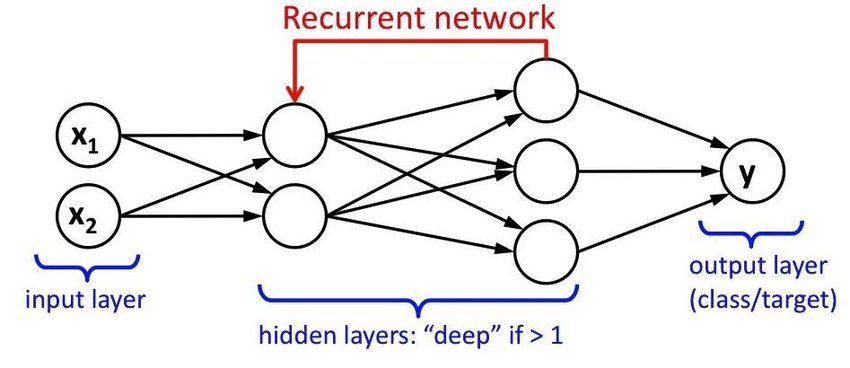
\includegraphics[width=\textwidth]{rnn}
    \caption{Een Recurrent Neural Network (RNN). Bron: \url{https://www.researchgate.net/figure/Recurrent-neural-networkRNN-or-Long-Short-Term-MemoryLSTM-5616_fig2_324883736}}
    \label{fig:rnn}
\end{figure}